\section{Design f"ur Analphabeten}
Das Standart Design von Anwendungen basiert meist auf Texte und die Benutzer sind vom Verstehen dieser Texte abh"angig. So  k"onnen Analphabeten schwer oder auch gar nicht diese Anwendungen verwenden. Außerdem haben Analphabeten durch ihre Leseschw"ache oft andere Herangehensweisen erlernt.\\
Um die Anwendung Analphabeten gerecht zugestalten gibt es zwei grundlegende M"oglichkeiten:
\begin{enumerate}
	\item Eine Variante die nur für funktionale Analphabeten geeignet ist, da hier weiterhin stark vereinfachte Texte verwendet werden.
	\item Diese Variante verzichtet auf jeden Text und ersetz diesen vollständig durch andere Medien, wie Bild und Ton.
\end{enumerate}

\subsection{Designentwicklung}\label{sec:designEval}
Um die Benutzerfreundlichkeit für Analphabeten zu überprüfen mussten neben den "ublichen "Uberpr"ufungen, ebenfalls Analphabeten als Testgruppen herangezogen werden. Die Testgruppen zum Analphabetismus sind Aufgrund ihrer Verschwiegenheit schwer zu finden. So empfielt es sich mit  Hilfsorganisationen wie \glqq alphabund \grqq zusammenarbeiten. Hier können auch oft bereits get"atigte Studien angefordert werden. Dabei stammen die Studien zu funktionalen Analphabeten vorwiegend aus den Industriestaaten und die Studien zu prim"aren und sekund"aren Analphabetismus meist aus Entwicklungsl"andern wie Indien und den Philippinen,  wie in der Studie aus dem Kapitel \ref{sec:beisp3}. Bei Testgruppen aus anderen L"andern m"ussen auch andere kulturelle Faktoren beachtet werden wie im Vortrag \glqq Design und Kultur \grqq, welche die Beobachtungen verf"alschen k"onnen.  \footnoteSource{\label{W.M.Gribbons01}William M. Gribbons}
					{Universal Accesibility and Low-Literacy Populations, Implications for Human-Computer, Interactions Desing and Research Methods}
					{2012}
					{The Human-Computer Interaction Handbook: Fundamentals, Evolving Technologies and Emerging Applications}
\footnoteSource{\label{MedhiSaraToyama01}Indrani Medhi, Aman Sagar, and Kentaro Toyama}
					{Text-Free User Interfaces for Illiterate and Semi Literate Users}
					{2006}{}
Bei der Arbeit mit den Analphabeten innerhalb der Studien, müssen die üblichen Schriftstücke wie Aufgabenliste oder Fragebogen ersetzt werden. Entweder sie werden durch Illustrationen oder Sprachaufnahmen ersetzt oder der Probant wird persönlich begleitet.
Da Analphabeten ge"ubt sind im Auswendig lernen von W"ortern und T"atigkeiten müssen die Probanten h"aufiger als "ublich ausgetauscht werden um zu gew"ahrleisten, dass die Anwendung tats"achlich Intuitiv ist.$^{\ref{W.M.Gribbons01}}$\\

\subsection{ Designfolgerungen}\label{sec:designClue}
Wie bereits erw"ahnt gibt es zwei grundlegende Varianten zum Design für Analphabeten.
\begin{itemize}
\item Das Verwenden von Bildern oder akustischen Ausgaben statt Texten für prim"are und sekund"are Analphabeten.
\item Das Vereinfachen und Unterst"utzen von Texten für eine breitere Benutzergruppe.
\end{itemize}
Die Variante für prim"aren und sekund"aren Analphabetismus unterscheidet sich haupts"achlich im vermeiden von Texten von der Variante für funktionale Analphabeten. Darum wird im Folgenden haupts"achlich auf die Variante für funktionale Analphabeten eingegangen.

Im Kapitel \glqq Universal Accesibility and Low-Literacy Populations, Implications for Human-Computer, Interactions Desing and Research Methods \grqq$^{\ref{W.M.Gribbons01}}$ aus dem Buch \glqq The Human-Computer Interaction Handbook: Fundamentals, Evolving Technologies and Emerging Applications \grqq beschreibt W.M.Gribbons die Folgerungen für das Design der Analphabeten in vier Kategorien:\\

\begin{itemize}
\item Lesen:              "Anderungen die das Lesen der einzelnen W"orter vereinfachen oder auch ersetzen.
\item Merken:            "Anderungen die das Merken vereinfachen und somit die Konzentration erh"ohen.
\item Metakognition: "Anderungen die zum Schlussfolgern und verstehen des Inhalts n"otig sind.
\item Suche und Navigation : "Anderungen die die Suche in der Anwendung und das Suchen von Informationen erleichtern.
\end{itemize}

\subsubsection{Lesen}\label{sec:designClueReading}
\begin{figure}[h]
	\centering
		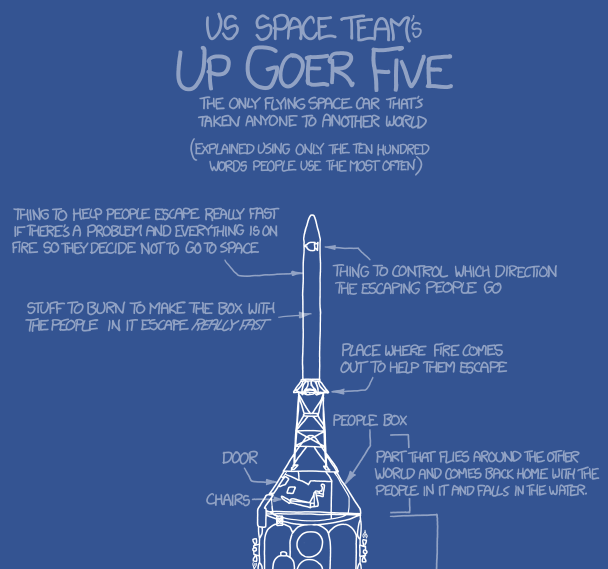
\includegraphics[width=0.50\textwidth]{Daten/up_goer_five_part.png}
	\caption{Up Goer Five: Einfache Sprache aber schwierige Schrift $^{\ref{up_goer_five_01}}$}
	\label{fig:GoerFive}
\end{figure}

Für prim"are und sekund"are Analphabeten, also Analphabeten die gar nicht lesen k"onnen, muss der Textinhalt vollst"andig durch andere Medien ersetzt werden. Neben einfachen Signalen wie Piept"onen k"onnen auch Tonaufnahmen oder Screenreader verwendet werden, wie im Vortrag zum Thema  \glqq Design für Menschen mit Sehsch"adigung \grqq vorgestellt.
Ebenfalls k"onnen Illustrationen verwendet werden, welche über ihren Bildinhalt die selben Informationen vermitteln.
Da Illustrationen aber wesentlich komplexer als Texte sind, müssen sie m"oglichst Aussagekr"aftig und leicht interpretierbar sein. Dabei sind auch wie aus dem Vortrag \glqq Globalisierung, Lokalisierung \grqq die kulturelle Unterschiede wichtig zu beachten.\\
Für funktionale Analphabeten muss der Text nicht zwingend ersetzt werden, doch ist es dann wichtig den Text einfacher und verst"andlicher zu gestalten. Damit wird dieser verst"andlicher für Analphabeten und sollte durch die bisher genannten alternativen Medien erg"anzt werden. Um das Lesen des Textes zu vereinfachen sollten die Informationen auf das wesentliche reduziert und in sinnvolle Gruppen gegliederdert werden. Auch hilft es den Text in einfacherer Sprache zu schreiben. Denn je nach verwendeten Wortschatz ist der Text einfacher oder auch schwerer zu verstehen. Ein Beispiel dazu ist in Abbildung \ref{fig:GoerFive} zu finden. Hier erkl"art Randall Munroe mit Hilfe der 1000 bekanntesten englischen W"orter den Aufbau der Saturn V Rakete.
\footnoteSource*{\label{up_goer_five_01}Jason Major}
				{This is Awesome: U.S. Space Team’s “Up Goer Five”}
				{5.6.2013}
				{http://www.universetoday.com/98411/this-is-awesome-u-s-space-teams-up-goer-five/}
 Durch die einfache Sprache f"allt es den Leser einfacher den Inhalt zu verstehen. Doch wurde eine ungünstige Schriftart verwendet, welche für ungeübte Leser schwerer zu lesen ist, denn auch die Schriftart beeinflusst die Schwierigkeit des Textes.
Um den Inhalt eines Textes zu Kategorisieren führten Croft und Peterson 2002 und Darrell West 2003 Arbeiten durch, in denen sie Schriftstücke verschieden schweren Wortsch"atzen zuordneten.
Demnach liegen etwa 70\% der Staatlichen Webseiten auf einem Level von 12 und Asthma bezogene Websites auf einem Level von 10.
Dabei verfügt die H"alfte der amerikanischen Bev"olkerung h"ochstens Level . Ein funktionaler Analphabet liegt noch weit darunter.
Ein Schriftstück von Level 8 kann somit von allen Amerikanern verstanden werden, ein Schriftstück mit niedrigeren Level jedoch auch von anderen Gruppen bis hin zu den funktionalen Analphabeten.$^{\ref{W.M.Gribbons01}}$\\

\subsubsection{Merken}
Merken hat nur indirekte Auswirkungen auf das Leseverhalten. Einerseits führen einige mentale Behinderungen die sich auf das Merken auswirken zum Analphabetismus wie auch schon im Vortrag \glqq Design für Menschen mit Lernschwierigkeiten \grqq angesprochen wurde. Andererseits kann eine Person nur eine bestimmte Menge an Konzentration aufwenden. Ist Diese bereits für das Merken verbraucht fehlt die Konzentration beim Lesen oder es werden Informationen vergessen und Passagen müssen erneut gelesen werden. Die F"ahigkeit zu Merken kann unterstützt werden indem die Informationen aufs wesentliche Reduziert werden oder in sinnvolle Gruppen gegliedert werden. Am wichtigsten ist jedoch, dass unn"otige Ablenkungen vermieden werden.
Die offensichtlichen Ablenkungen sind blinkende Werbebanner oder Lauftext, aber auch zu viele Nebenaufgaben lenken stark von der Hauptaufgabe ab und sollten m"oglichst reduziert werden. Denn mit vielen Aufgaben muss nicht nur mehr Informationen gemerkt, sondern auch der Informationswert für die einzelnen Aufgaben ermittelt werden. Für den Inhalt selber ist es wichtig, dass Widersprüche m"oglichst vermieden werden. Denn Widersprüche zwingen den Benutzer die Informationen erneut durch zugehen und zu bewerten und zwingen ihn die Kapitel erneut zu lesen.

\subsubsection{Metakognition}
\begin{figure}[h]
	\centering
		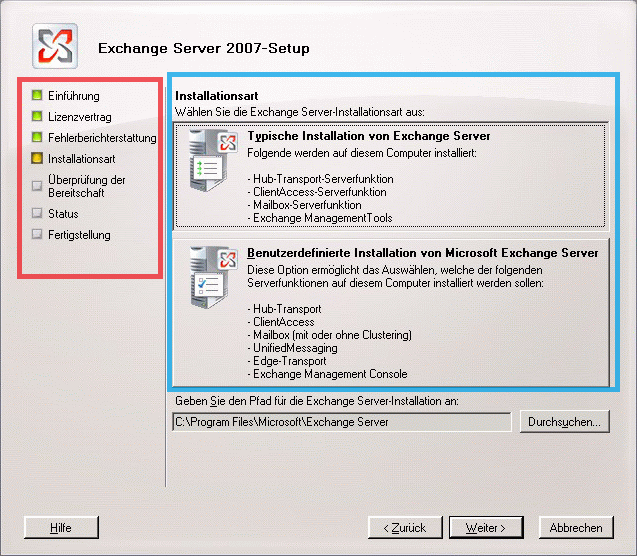
\includegraphics[width=1.00\textwidth]{Daten/ServerBeispiel.png}
	\caption{Interface mit Checkliste und Wahlm"oglichkeiten $^{\ref{mc_serv_01}}$}
	\label{fig:InstallBsp}
\end{figure}
Die Metakognition beschreibt das Verarbeiten und Kombinieren der gesammelten Informationen und überschneidet sich in einigen Punkten mit den anderen Kategorien. Um die Metakognition zu verbessern sollte die Anwendung möglichst einheitlich gehalten werden, damit der Benutzer sich selten in neue Bedienungen einfinden muss. Um das Zielsetzen zu erleichtern, kann die Anwendung bereits das Zeil vorgeben. So sieht der Benutzer z.b. das er sich erst Anmelden muss. Auch kann eine Übersicht der Ziele mit zukünftigen und bereits abgechlossenen Zielen in Form einer Checkliste sinnvoll sein. Ein Beispiel für solche Checklisten ist die Installationssoftware vom Microsoft-Server 2007
\footnoteSource{\label{ mc_serv_01}Microsoft}
						{Microsoft-Server 2007 Installation}
						{Stand : 14.2.2013}
						{http://i.technet.microsoft.com/dynimg/IC22550.gif} 
aus der Abbildung \ref{fig:InstallBsp}. Hier Rot markiert sind die einzelnen Installationsschritte w"ahrend der gesamten Installation einsehbar.\\
Auch eine Men"u oder eine einfache Auswahl kann sehr fordernd für Analphabeten sein. Diese Wahlmöglichkeiten sollten möglichst eindeutig sein, dabei aber auch nicht zu kompliziert Beschrieben sein. Da dies meist nicht der Fall ist, verwenden Analphabeten h"aufig
einfach die erste M"oglichkeit. In manchen Fällen kann dieses Verhalten ausgenutzt werden, indem man diese Auswahl f"ur Analphabeten optimiert. So kann im Beispiel aus der Abbildung \ref{fig:InstallBsp}mit Blau markiert, die Auswahl über den Installationsumfang getroffen werden. Die erste Variante bietet hier eine vordefinierte Auswahl und ist somit Ideal für einen Analphabeten..$^{\ref{W.M.Gribbons01}}$\\


\subsubsection{Navigation und Suche}
\begin{figure}[h]
	\centering
		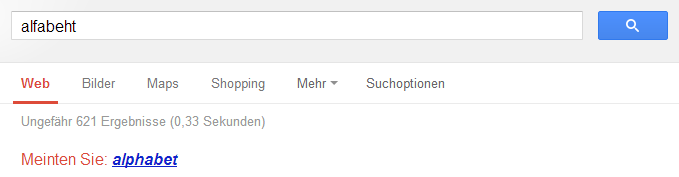
\includegraphics[width=0.80\textwidth]{Daten/rechtschreibung.png}
	\caption{Fehlerkorrektur der Suche bei Google $^{\ref{google01}}$}
	\label{fig:GoogleSearch}
\end{figure}

Übersicht ist für jeden Benutzer sinnvoll. Jedoch ist es schwer die Balance zwischen vielen Wahlm"oglichkeiten und der Tiefe der Wahlm"oglichkeiten zu finden. Gerade zum Unterscheiden der M"oglichkeiten sollte klar sein, wohin welche Auswahl führt, damit sich
 die Suchwege m"oglichst verkürzen. Eine weitere Variante um den Suchweg zu verkürzen ist den Verlauf anzuzeigen, damit der Benutzer zurück verfolgen kann was er bereits bearbeitet hat. Ebenso sollten die wichtigsten oder auch h"aufigsten Inhalte wie Suche, Anmelden und Hilfe m"oglichst ohne suchen zug"anglich sein.\\
Die Suche stellt für Analphabeten eine besondere Herausforderung dar. Die übliche Suche ben"otigt eine genaue Eingabe des zu suchenden Wortes. Da aber Analphabeten h"aufig die W"orter falsch schreiben kommen sie gew"ohnlich nicht an das gewünschte Ziel. Darum sollte die Suche die Eingabe erst interpretieren und gegebenenfalls Alternativen anbieten.
Als g"angigstes Beispiel hierfür dient die Suchmaschiene Google$^{\ref{fig:GoogleSearch}}$, welche z.B. als Korrektur für \glqq alfabeht \grqq \glqq alphabet\grqq angibt.
\footnoteSource{\label{google01}Google Inc.}
						{Google Suchmaschiene}
						{Stand : 5.6.2013}
						{www.google.de}

\subsection{Beispiele: Design für Analphabeten}
In diesem Kapitel folgen drei Beispiele für Anwendungen die für Analphabeten geeignet sind und die in \ref{designClue} genannten Kriterien verdeutlichen sollen. Dabei würden m"oglichst verschiedene Anwendungen gew"ahlt, um zu zeigen auf welche unterschiedlichen Weisen Anwendungen für Analphabeten funktionieren k"onnen..$^{\ref{W.M.Gribbons01}}$\\


\subsubsection{ integrierte Software: ReadSpeaker}

Dieses Beispiel ist eine integrierte Software, welche beliebigen Text der Website Bundesverband Alphabetisierung
\footnoteSource{\label{alphaBund01}Bundesverband Alphabetisierung}
						{Bundesverband Alphabetisierung Website}
						{Stand : 14.2.2013}
						{http://www.alphabetisierung.de/}
vorlesen kann.
Dabei markiert der Benutzer den zu "ubersetzenden Text, worauf unten rechts eine Schaltfl"ache \glqq Vorlesen \grqq wie in Abbildung  \ref{fig:DesignBeispiel1} erscheint. Mit dieser kann nun die Wiedergabe gestartet werden, worauf wieder eine weitere Schaltfl"ache erscheint, mit der unter anderem die Wiedergabe gestoppt oder pausiert werden kann.\\
Somit wird der Umfang der Website für funktionale Analphabeten weit gesteigert und auch andere Analphabeten dürften sp"atestens nach einer kleinen Einweisung den Umfang nutzen k"onnen. Auch ist nur die Maus als Eingabeger"at n"otig. So kann eine Beliebige Seite mit beliebigen Inhalt für den Anbieter leicht den Analphabeten zug"anglich gemacht werden. Dabei kann bis auf in Bildern vorkommender Text, jeder Text ohne Teure Tonaufnahmen übersetzt werden, wie in \ref{sec:designClueReading}. Dabei geht aber die Übersichtlichkeit verloren, da es für den Benutzer dauert den Text zu markieren und anzuh"oren. Außerdem ist der Wortschatz nicht unbedingt für Analphabeten geeignet und durch den Übersetzter schwer zu verstehen.
\begin{figure}[h]
	\centering
		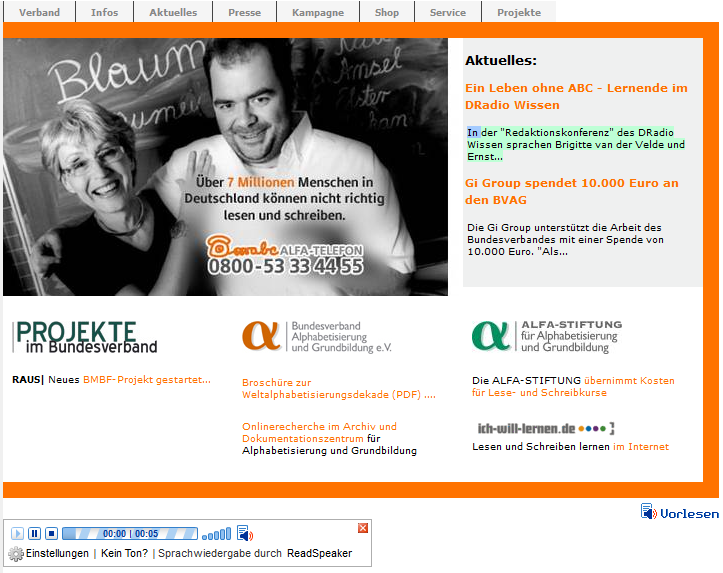
\includegraphics[width=0.80\textwidth]{Daten/DesignBeispiel1.png}
	\caption{Design Beispiel vom Bundesverband Alphabetisierung $^{\ref{alphaBund01}}$}
	\label{fig:DesignBeispiel1}
\end{figure}

\newpage

\subsubsection{Reines Text-Design : Inisque}
In diesem Beispiel kommen wir zu einer Anwendung, welche nur für funktionale Analphabeten entwickelt wurde: Die Suchmaschine Invisque (INteractive VIsual Search and QUery Environment)
\footnoteSource{\label{Invisque01}Invisque - INteractive VIsual Search and QUery Environment}
						{Stand: 5.6.2013}
						{http://www.invisque.com/index.html}{}
.\\
Diese Suchmaschine ist in erster Linie nicht nur für Analphabeten entwickelt worden, aber wurde laut Angaben der Entwickler so weiterentwickelt, dass sie auch für funktionale Analphabeten geeignet ist. Um dieses Ziel zu erreichen, haben die Entwickler versucht einige Probleme, die funktionale Analphabeten haben, entgegen zu wirken, wie das es diesen Menschen schwer f"allt sich auf den Text zu konzentrieren, wenn sehr viel ablenkender weiterer Text auf der Seite verteilt wird, oder wenn PopUps auftauchen, oder Werbung allgemein an den R"andern blinkt. All dies blendet Invisque erfolgreich mit einer Blanko-Oberfl"ache aus. Invisque verwendet einen wenig irritierenden weißen Hintergrund, in den Ecken befinden sich kleine Felder, aus denen weitere Informationen und Navigationsunterstützung gew"ahlt werden k"onnen. wie auf Abb.\ref{fig:Invisque} zu sehen ist.

\begin{figure}[h]
	\centering
		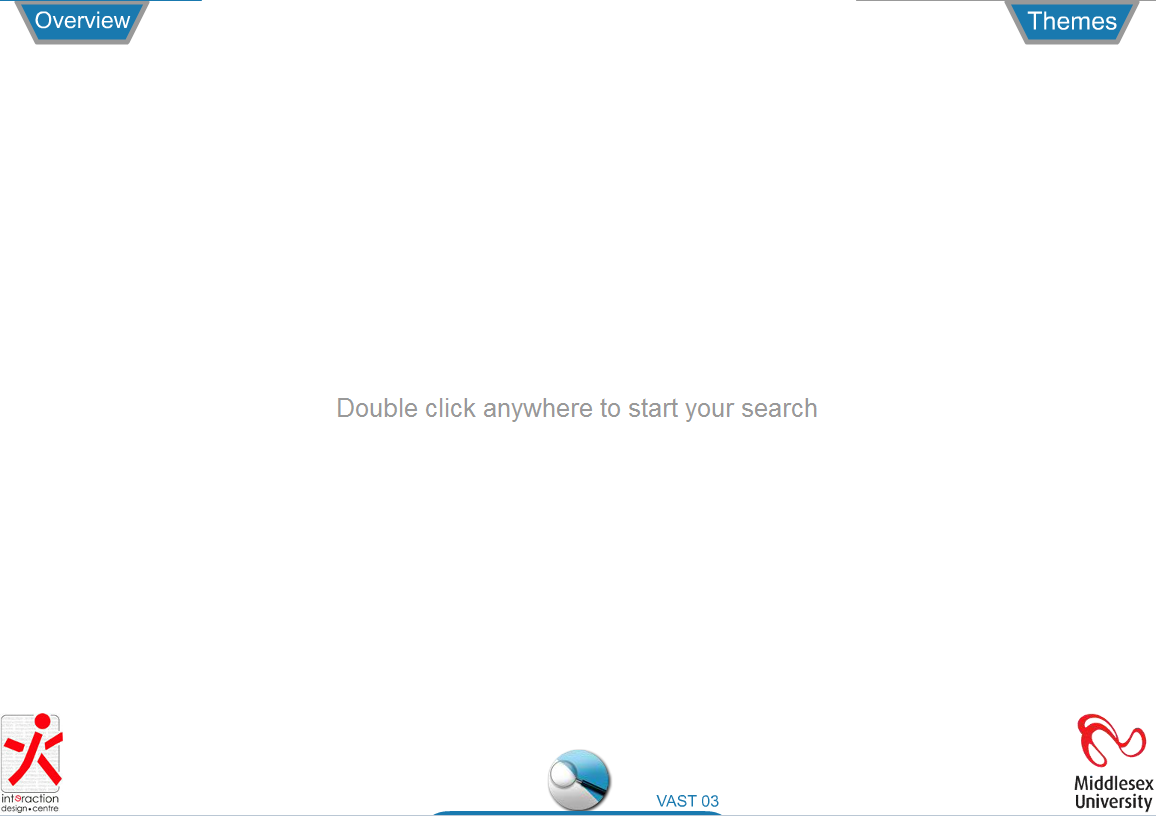
\includegraphics[width=0.80\textwidth]{Daten/Inisque.PNG}
	\caption{Invisque Oberfl"ache}
	\label{fig:Invisque}
\end{figure}

Um einen guten Überblick über diese Suchmaschine zu bekommen, ist es zu empfehlen sie selbst Auszuprobieren und verschiedene Schlüsselw"orter einzugeben.

\newpage
\subsubsection{textlose Anwendung}\label{sec:beisp3}
In diesem Beispiel geht es um zwei Anwendungen welche zur Studie \glqq Text-Free User Interfaces for Illiterate and Semi Literate Users \grqq
\footnoteSource{\label{MedhiSagarKentaro01}Indrani Medhi, Aman Sagar, and Kentaro Toyama}
					{Text-Free User Interfaces for Illiterate and Semi Literate Users}
					{2006}
					{}
 von Indrani Medhi, Aman Saga und Kentaro Toyama geschrieben wurden.\\
Ziel war es Anwendungen zu schreiben, welche einer Indischen Slumbev"olkerung eine erleichterte Jobsuche und eine Wegbeschreibung bieten sollten. Da diese Bewohner oft bei ihrem Job bleiben und ihn nicht mehr so leicht auf geben , auch wenn der Lohn, den sie dafür erhalten viel zu niedrig ist und sie die Chance h"atten, einen besseren Job zu bekommen. Diese Bev"olkerung besteht zum gr"oßten Teil aus prim"aren Analphabeten, dabei mussten die Entwickler nicht nur mit den Analphabeten üblichen Problemen wie in \ref{sec:designEval} k"ampfen, sondern auch viel mit den Kulturellen. Zum Beispiel hatte kaum ein Bewohner bisher Erfahrung mit digitaler Technik.\\
Besonders wurden die Interpretationen der Bilder hervorgehoben. Bilder die die Entwickler eindeutig fanden, waren für die Bev"olkerung noch lange nicht zu verstehen. So mussten für Abspülen und Kochen extra noch Feuer und Wasser hinzugefügt werden, wie man in Abbildung \ref{fig:picfail} sehen kann. (Zur Veranschaulichung haben wir das Bild um die Illustrationen ohne Feuer und Wasser erweitert.) Hier wurden die linken Darstellungen eher als Geschirr angesehen, statt den gewollten Aktionen Abspülen und Kochen. Somit wurden sie durch die rechten Darstellungen ersetzt.\\\\

\begin{figure}[h]
	\centering
		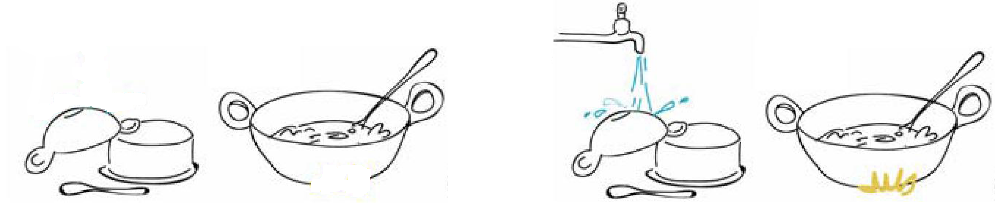
\includegraphics[width=1.00\textwidth]{Daten/pic_fail2.PNG}
	\caption{Deutlichkeit der Illustrationen $^{\ref{MedhiSagarKentaro01}}$}
	\label{fig:picfail}
\end{figure}

Die erste Anwendung soll den Benutzer eine Karte bieten um zu seinem Zielort zu kommen, wie in Abbildung \ref{fig:mapsimple}.\\
Übliche Karten arbeiten mit Straßennamen, welche einen Analphabeten jedoch nicht weiterhelfen. Somit soll hier der Benutzer sich an Merkmalen der Straßen wie Gesch"aften ,Krankenh"auser oder Bushaltestellen zurechtfinden.
Bei der ersten Version dieser Anwendung wurde die Person als Pfeil und die zu gehende Wege in Blau markiert. Jedoch führte das zu Missverst"andnissen mit den Probanten. So wurde der Weg als Fluss und der Pfeil erst gar nicht wahrgenommen. Darum ersetzten die Entwickler die Straßen in Grau und den Markierten Weg durch einen dunkleren grau Ton und einem verbreiterten den Weg markiert.
Auch der Pfeil wurde durch eine Figur ersetzt, welche je nach Richtung entweder von Vorne, hinten oder der Seite zu sehen ist.

\begin{figure}[h]
	\centering
		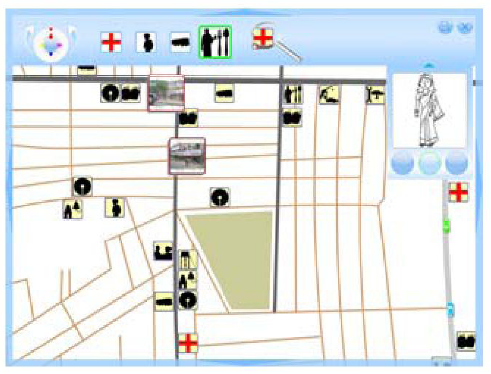
\includegraphics[width=0.8\textwidth]{Daten/map_simple.PNG}
	\caption{Vereinfachte Karte $^{\ref{MedhiSagarKentaro01}}$}
	\label{fig:mapsimple}
\end{figure}
Die zweite Anwendung soll dem Benutzer eine Art Job-B"orse bieten und somit einen besseren Anschluss an die restliche Bev"olkerung bieten.\\
Dabei wird ebenfalls vollst"andig auf geschriebenen Text verzichtet, sodass Analphabeten leicht mit der Anwendung umgehen k"onnen.
Was allerdings nicht auf den folgenden Abbildungen zu sehen ist, ist die Sprachausgabe die über die Hilfe zu jeder Information m"oglich ist. Klickt der Benutzer auf die Hilfe wird zur jeweiligen Ansicht die n"otigen Informationen und Verwendungs-M"oglichkeiten erz"ahlt.
In der ersten Abbildung \ref{fig:joblist} ist zusehen wie die Anwendung nur aus Bildern besteht. Zusehen ist eine Liste von Jobs, wie der Benutzer zu dieser Auswahl gelangt oder wodurch Sie bestimmt wird wurde nicht erw"ahnt.\\
Das Stadt "ahnliche Symbol links soll zeigen, ob der Arbeitsplatz in der Stadt liegt oder nicht. In der Mitte sind die geforderten Aufgaben zuerkennen. Danach wird die für den Ort übliche Uhr als Zeitangabe mit Mond und Sonne als Zeichen für Vor- und Nachmittags dargestellt. Da in der Studie beobachtet wurde, dass die Probanten keine Probleme mit Zahlen hatten, wird ganz rechts der Lohn als Geldschein mit dem Wert angezeigt.\\
Die Hilfe ist über das Portrait zu finden, da es den meisten Probanten leicht viel ein Portrait einer beliebigen Person als Hilfe wahrzunehmen. Um nun eine detailiertere Ansicht des Berufs zu erhalten muss der Proband nur auf die passende Reihe klicken und kommt so zu Abbildung \ref{fig:jobclose}.
Hier sind die Informationen noch einmal genauer aufgeführt. Oben in der Mitte wird die Arbeitszeit nun auch mit Ende, bzw. mit Unterbrechung angegeben. Der Lohn steht nun auch in tats"achlichen Geldscheinen in der rechten Ecke. Auch steht nun bei jeder T"atigkeit dabei, welchem Lohn sie entspricht, damit der Bewerber den Aufwand erkennen kann. Zum Schluss finden sich unten die Angaben in welchen und wie vielen R"aume was zu tun ist.

\begin{figure}[h]
	\centering
		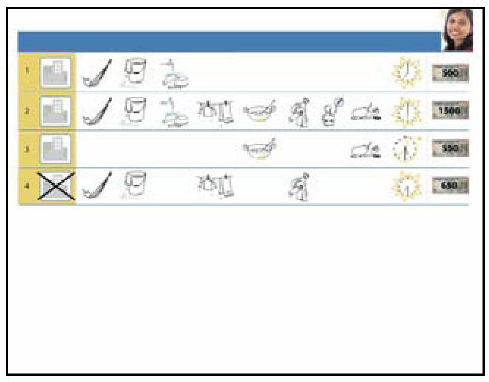
\includegraphics[width=0.90\textwidth]{Daten/job_list.PNG}
	\caption{Job Liste basierend auf Bildern $^{\ref{MedhiSagarKentaro01}}$}
	\label{fig:joblist}
\end{figure}


\begin{figure}[h]
	\centering
		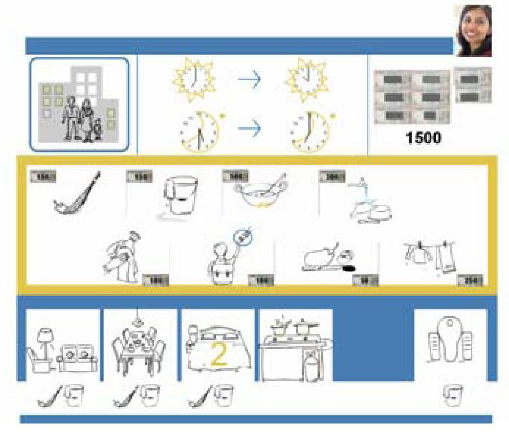
\includegraphics[width=0.8\textwidth]{Daten/job_close.PNG}
	\caption{Job Ansicht $^{\ref{MedhiSagarKentaro01}}$}
	\label{fig:jobclose}
\end{figure}

\clearpage
